\section{Preprocessing and performance}
\label{sec:preprocessing}

In the following, we assume all ``raw'' light curves to be median normalized, and each light curve segment to be obtained from splitting this median normalized light curve into parts. The first preprocessing step we take is centering the light curve segments by subtracting 1.  Additionally, we investigate the effect of scaling the light curves by their estimated noise level $\sigma$, so the network performance becomes less dependent on this noise and instead more on the transit depth relative to this noise. We will refer to this as sigma scaling.

\begin{figure}
    \centering
    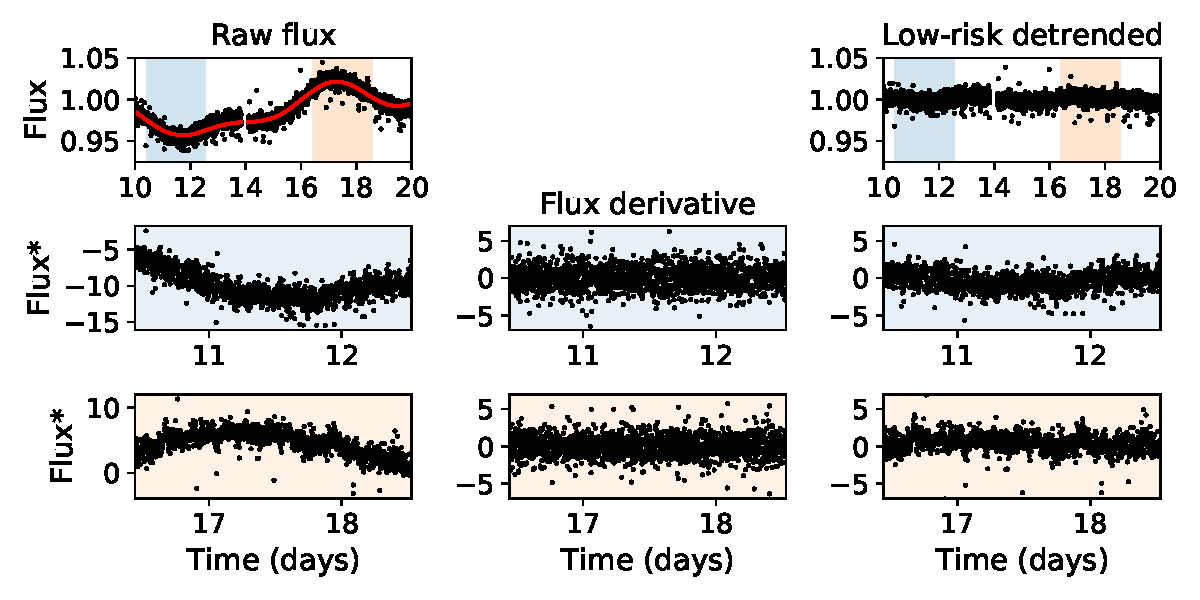
\includegraphics[width=0.7\linewidth]{Experiments/Figures/Preprocessing/input-range-example.pdf}
    \caption{(Left) Two segments are taken from a ``raw'' median normalized light curve, which have considerably different flux ranges after preprocessing. (Middle) Taking the derivative solves the problem of different input ranges, while conserving all relevant information. (Right) With loss of information, one could carefully remove large-scale trends in the light curve, i.e. the red trend line in the top-left panel, to achieve a similar result.}
    \label{fig:input_ranges}
\end{figure}

Still, the range of flux values might greatly vary between two separate light curve segments, as illustrated in Figure \ref{fig:input_ranges}. This is understood by realizing that the original light curve may contain large-scale fluctuations due to stellar rotation modulation. The network might interpret these range differences as indicators of the presence of a transit signal, in particular if there is little data available for a certain range of flux values. This is not what we want, because a transit event can occur at any given time, independent from the activity on the stellar surface. Applying median normalization again to the segments is not a solution, because then we prevent the network from learning to deal with input ranges it would normally encounter in full-length light curves. An alternative which avoids this problem, is to take the derivative of the input light curve and feed it to the network instead of the absolute values.

\begin{figure}
    \centering
    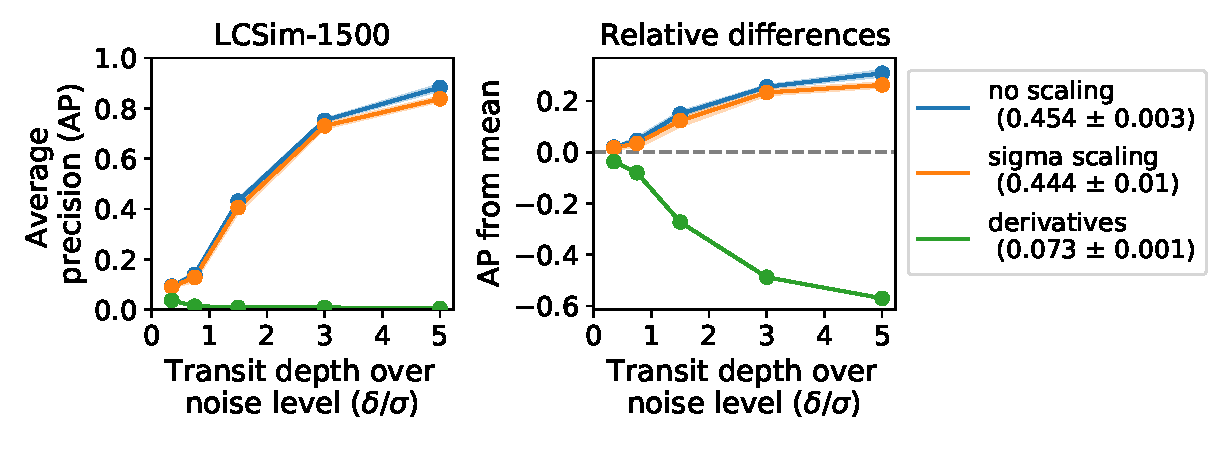
\includegraphics[width=0.7\linewidth]{Experiments/Figures/Preprocessing/lcsim1500_AP_pp-basic.pdf}
    \caption{The average precision of the RNN evaluated at different transit depth bins for different basic preprocessing steps. At larger depths, the AP is expected to be higher. The right figure shows the deviations from the mean of all curves. Filled regions, which are narrow in this figure, show one standard deviation over the results of three differently initialized networks applied to the LCSim-1500 test split. Values between brackets in the legend show the overall AP and standard deviations over three runs.}
    \label{fig:lcsim_pp_basic}
\end{figure}

\begin{figure}
    \centering
    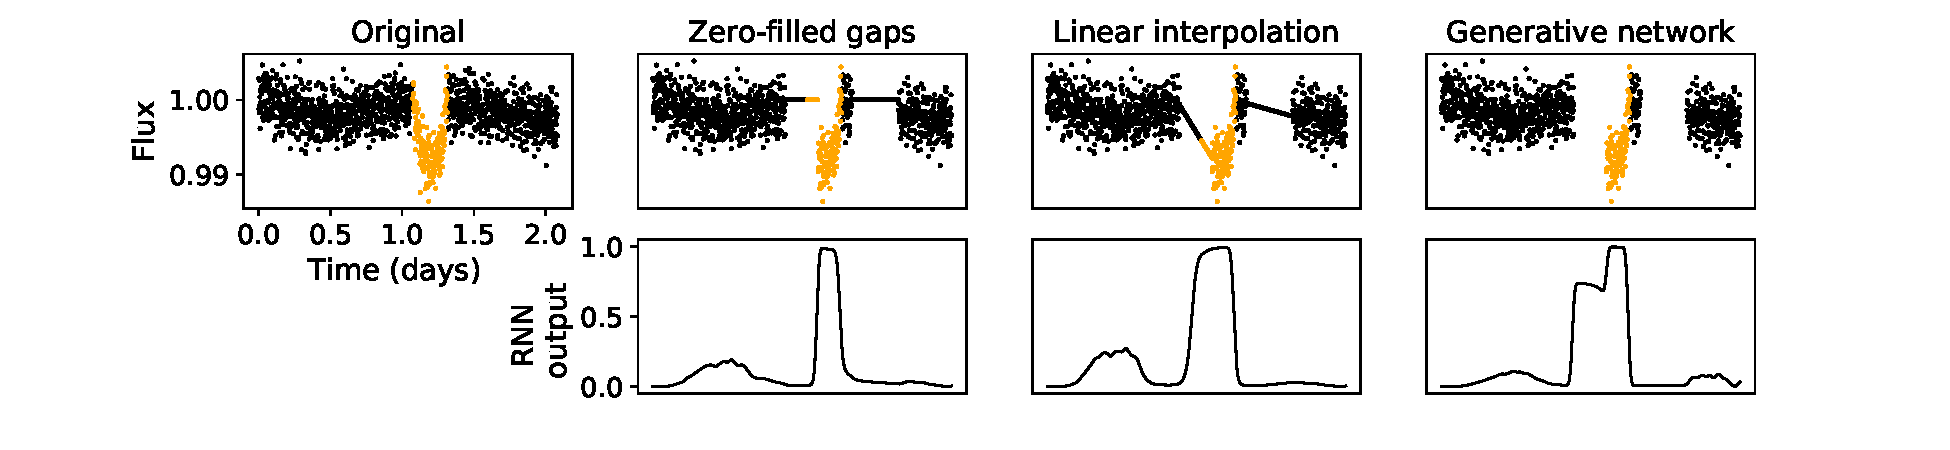
\includegraphics[width=\linewidth]{Experiments/Figures/Preprocessing/gap_examples.pdf}
    \caption{An example from the LCSim-1500-Gap validation split, with different approaches to dealing with gaps and the corresponding PTS of the RNN, i.e. the RNN's outputs at every time step. The signal data points are indicated by orange. Zero-filling in this example translates to one-filling, because the light curve segments are centered around zero before they are fed to the RNN.}
    \label{fig:gap_examples}
\end{figure}

\begin{figure}
    \centering
    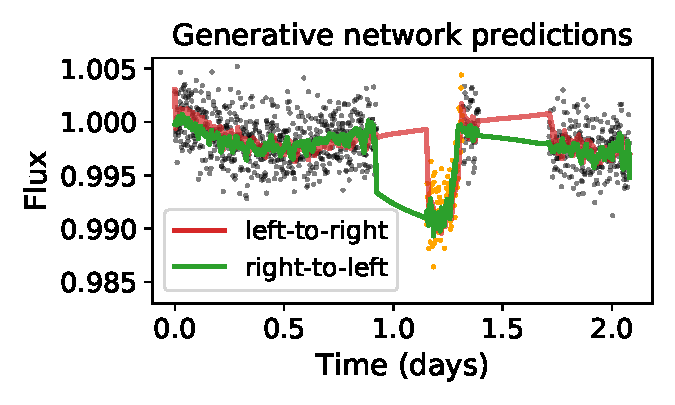
\includegraphics[width=0.35\linewidth]{Experiments/Figures/Preprocessing/generative-rnn_predictions.pdf}
    \caption{The predicted flux values visualized with red and green from the bidirectional generative RNN corresponding to the right-most figure in Figure \ref{fig:gap_examples}. The network seems to follow an expected trend in both directions, however, the gaps are not filled in a satisfactory manner.}
    \label{fig:generative_preds}
\end{figure}

Figure \ref{fig:lcsim_pp_basic} shows the effect of these different preprocessing steps on the AP of the RNN in the task of classifying individual data points as signal or non-signal. In this figure, we can observe a small difference between using no scaling and using sigma scaling, in favor of no scaling. We found that using derivatives instead of absolutes prevents the network from learning\footnote{In an earlier iteration of this work when less complex data was used (e.g. with less stellar variability), the derivative inputs worked well. Only with increased complexity the model started to fail.}.

To deal with gaps, we compare two gap-filling approaches and the use of the generative RNN. The gap-filling approaches are simple as we do not aim to reconstruct the original light curve, but rather produce an input that the RNN can handle well. Figure \ref{fig:gap_examples} visualizes how each approach works, and Figure \ref{fig:generative_preds} visualizes the predictions of the generative RNN applied to the same example. Since we use a bidirectional RNN, we get two streams of predictions. We can see from the figures that this creates some unrealistic artefacts in the predicted curve, which is likely the cause for the bumped peak in the PTS of the generative RNN. Therefore unexpectedly, we found that the generative network slightly outperformed the other two approaches when applied to a larger data set, especially for the shallowest transit signals. The results are plotted in Figure \ref{fig:lcsim_gaps}. The second best approach tested was linear interpolation, and the worst was zero-filling. In terms of efficiency, linear interpolation is preferred over the generative RNN. This is because during training, the generative RNN needs to evaluate at each time step whether the data point is missing, and if so, replace it with its own prediction before it proceeds to the next time step. This, in combination with the fact that we could not use pre-implemented RNN architectures in PyTorch for this purpose, resulted in an increase of training time of more than five times compared to the standard RNN applied to linearly interpolated data.

\begin{figure}
    \centering
    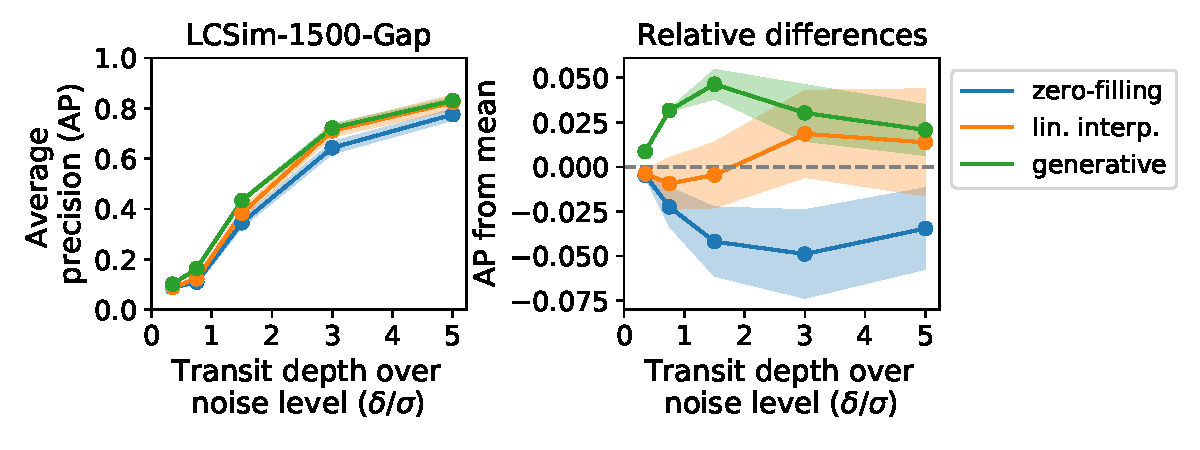
\includegraphics[width=0.7\linewidth]{Experiments/Figures/Preprocessing/lcsim1500_AP_pp-gaps.pdf}
    \caption{The average precision for varying transit depths, with filled regions indicating the standard deviation of three runs on the test split of LCSim-1500-Gap with differently initialized networks. The comparison includes different methods to deal with data gaps: filling gaps with zeros, linear interpolation, or using predictions from the generative RNN. }
    \label{fig:lcsim_gaps}
\end{figure}

In Figure \ref{fig:lilith_pp_basic}, we evaluate a subset of the same preprocessing steps applied to the Lilith-1500 data set. In the shallower transit range, it appears that sigma scaling results in worse performance than no scaling. However, for deeper transits the difference between the scaling approaches becomes larger, in favor of sigma scaling. From the figure it also seems that zero-filling is the better approach to deal with data gaps, in contrast to our earlier results.
\begin{figure}
    \centering
    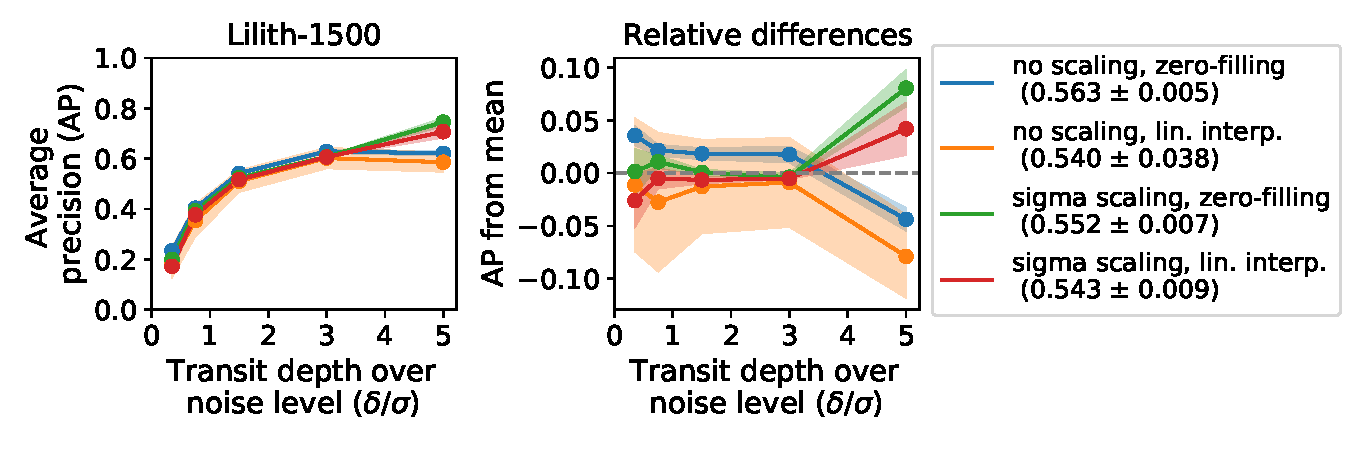
\includegraphics[width=0.78\linewidth]{Experiments/Figures/Preprocessing/lilith1500_AP_pp-basic-gaps.pdf}
    \caption{The effect of different basic preprocessing steps on the performance of the RNN applied to Lilith light curve segments. Filled regions indicate the standard deviation over three runs using differently initialized models that were applied to the test split after training. Values between brackets show the overall AP.}
    \label{fig:lilith_pp_basic}
\end{figure}



Lastly, we evaluate additional preprocessing steps applied to Lilith light curves. First of all, to address the problem illustrated in Figure \ref{fig:gap_examples}, we detrend the original light curves (before segmenting) with a filter that only removes the largest trends. We refer to this as low-risk detrending (LRD). For this, a Savitzky-Golay filter was used with a polynomial order of 2 and a window length of 2881, i.e. $\sim$4 days (see \citealp{hippke2019wotan} for details on the implementation of the Savitzky-Golay filter). We also test the effect of detrending the original light curve with a filter that would more commonly be used in combination with other search algorithms. We refer to this as high-risk detrending (HRD). For this, a time-windowed sliding median filter was used with a window length of 12 hours. Another preprocessing step is that of removing outliers. In the comparison, we test the effect of removing outliers above 6$\sigma$ and below 12$\sigma$ from the median of a sliding 30-minute window, to avoid clipping out transit signals. Finally, since Lilith provides centroid data, we investigate the effect of using the centroids as additional input to the network at each time step. The results shown in Figure \ref{fig:lilith_pp_advanced} show that outlier removal resulted in worse performance. This is possibly due to the fact that removing outliers creates missing data which need to be imputed. The results also show that LRD and centroid inputs are beneficial to the network, although there is some overlap between different runs. In the mid-range of transit depths, LRD and centroid inputs seem to be consistently better than other methods. Furthermore, without detrending the network is still able to perform comparably to using HRD and LRD, which underlines our claim that the RNN does not require its inputs to be cleared of short-scale time-dependent noise in order to do its task.

In each of the following experiments, we make use of sigma scaling and linear interpolation in case the data contains gaps.
\begin{figure}
    \centering
    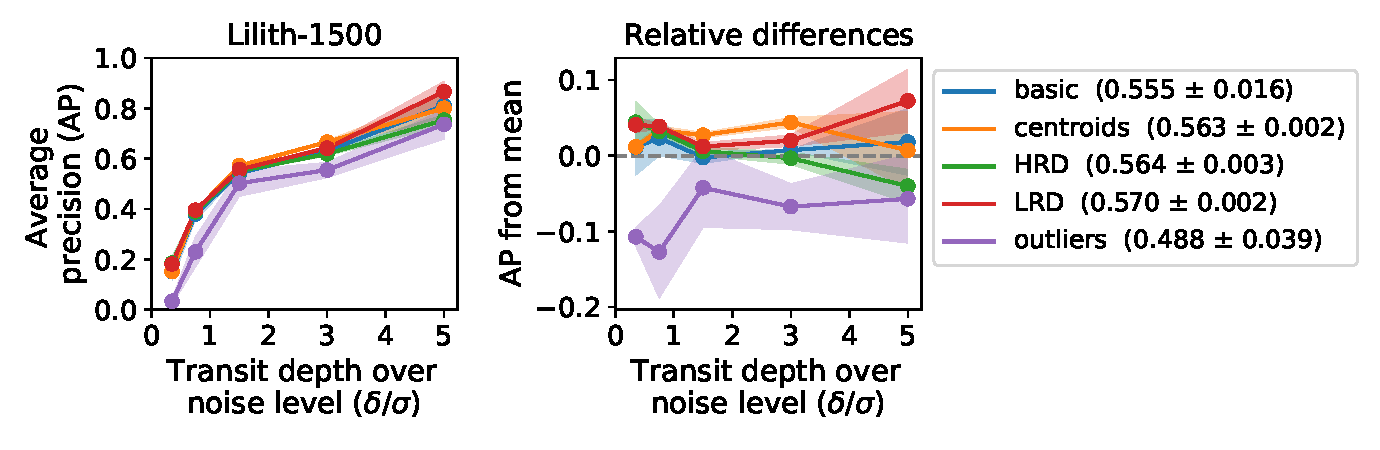
\includegraphics[width=0.79\linewidth]{Experiments/Figures/Preprocessing/lilith1500_AP_pp-advanced.pdf}
    \caption{The effect of high- and low-risk detrending, centroid inputs and outlier removal on the average precision of the RNN, in comparison with only using basic preprocessing, i.e. sigma scaling and linearly interpolating data gaps. The results are obtained on the test set of Lilith-1500. Standard deviations over three runs are indicated by the filled regions.}
    \label{fig:lilith_pp_advanced}
\end{figure}
